\documentclass[]{article}

% Imported Packages
%------------------------------------------------------------------------------
\usepackage{amssymb}
\usepackage{amstext}
\usepackage{amsthm}
\usepackage{amsmath}
\usepackage{enumerate}
%\usepackage{fancyhdr}
\usepackage[margin=1in]{geometry}
\usepackage{graphicx}
%\usepackage{extarrows}
%\usepackage{setspace}
\usepackage{float}
\usepackage[hidelinks]{hyperref}

% Configure Packages
%------------------------------------------------------------------------------
\hypersetup{linktoc=all}
\graphicspath{{Resources/}}
%------------------------------------------------------------------------------

% Header and Footer
%------------------------------------------------------------------------------
\pagestyle{plain}

\begin{document}
\cleardoublepage
\pagenumbering{gobble}
\begin{titlepage}
	\newcommand{\HRule}{\rule{\linewidth}{0.5mm}} % Defines a new command
	%for the
	%horizontal lines, change thickness heReve
	\center % Center everything on the page

	%----------------------------------------------------------------------------------------
	%	HEADING SECTIONS
	%----------------------------------------------------------------------------------------

	\textsc{\LARGE McMaster University}\\[1.5cm] % Name of your
	%university/college
	\textsc{\Large Software Design II \\  \Large Large System Design}\\[0.5cm] % Major heading
	%such as course name
	\textsc{\large SFWR ENG 3A04}\\[0.5cm] % Minor heading such as course
	%title

	%----------------------------------------------------------------------------------------
	%	TITLE SECTION
	%----------------------------------------------------------------------------------------

	\HRule \\[0.4cm]
	{ \huge \bfseries Deliverable \# 3}\\[0.4cm] % Title of your
	%document
	\HRule \\[1.5cm]

	%----------------------------------------------------------------------------------------
	%	AUTHOR SECTION
	%----------------------------------------------------------------------------------------

	\Large \emph{Authors:}\\
	Alexander \textsc{Jackson} \textbf{1302526} \\
	Harit \textsc{Patel} \textbf{1317372} \\ %Add your student number
	Josh \textsc{Voskamp} \textbf{1319352} \\
	Lucas \textsc{Bongers} \textbf{1202472} \\
	Mohammad \textsc{Naveed} \textbf{1332196} \\[3cm]
	%----------------------------------------------------------------------------------------
	%	DATE SECTION
	%----------------------------------------------------------------------------------------

	{\large \today}\\[3cm] % Date, change the \today to a set date if you
	%want to be precise

	\vfill % Fill the rest of the page with whitespace

\end{titlepage}

% Table of Contents
% Start numbering pages after ToC
\tableofcontents
\cleardoublepage
\pagenumbering{arabic}

\section{Introduction}
\label{sec:introduction}
% Begin Section


\subsection{Purpose}
\label{sub:purpose}
% Begin SubSection

The purpose of this document is to provide the developers with a more detailed design of the system-to-be. Furthermore, this document also includes diagrams that provide insight on system states and classes. The intended audience for this document are the developers, TA's, and Dr. Khedri.

% End SubSection

\subsection{System Description}
\label{sub:system_description}
% Begin SubSection

The application will identify land animals by presenting a series of questions to the user. The application will then produce a list of known animals that best match the answers entered by the user. With each possible match, the application will display basic information about the animal as well as a link to a webpage where the user can find more detailed information. In addition, the application will retain a list of recent animals spotted by the user, including marking on Google Maps the location of the user when each animal was sighted.
\\
\\
The application is designed to run on an Android smart-phone. The application will require the use of the Google Maps API, and will depend on the smart-phone having Internet access and location permissions. The application is designed to be self-contained and will not access any files on the device other than its own.

% End SubSection

\subsection{Overview}
\label{sub:overview}
% Begin SubSection

The rest of this document contains information about the detailed design of the application and its classes. Section 2 of this document features a state chart for each controller class of the application, and section 3 contains a sequence diagram for each use case of the application. Section 4 provides a detailed class diagram for the application. The final section of this document is a division of labour table that indicates the contributions of each individual to this document.

% End SubSection

% End Section

\section{State Charts for Controller Classes}
\label{sec:state_charts_for_controller_classes}
% Begin Section
\begin{figure}[H]
	\addcontentsline{toc}{figure}{GUI controller}
	\centering
	\includegraphics[width = 14cm]{GUIControlStateChart}
	\caption{State Chart Diagram for GUI controller}
	\label{State Chart Diagram for GUI controller}
\end{figure}

\begin{figure}[H]
	\addcontentsline{toc}{figure}{Animal Identification Controller}
	\centering
	\includegraphics[width = 7cm]{IdentificationStateChart}
	\caption{State Chart Diagram for Animal Identification Controller}
	\label{State Chart Diagram for Animal Identification Controller}
\end{figure}

\begin{figure}[H]
	\addcontentsline{toc}{figure}{Each Expert Controller}
	\centering
	\includegraphics[width = 7cm]{ExpertStateChart}
	\caption{State Chart Diagram for each Expert, i Controller}
	\label{State Chart Diagram for each Expert, i Controller}
\end{figure}

% End Section

\section{Sequence Diagrams}
\label{sec:sequence_diagrams}
% Begin Section
%This section should provide a use case diagram for your application.
\begin{figure}[H]
	\addcontentsline{toc}{figure}{Identify Animal}
	\centering
	\includegraphics[width = 14cm]{IDAnimalSequenceDiagram}
	\caption{Identify Animal Sequence Diagram}
	\label{Identify Animal Sequence Diagram}
\end{figure}

\begin{figure}[H]
	\addcontentsline{toc}{figure}{Select Experts}
	\centering
	\includegraphics[width = 7cm]{SelectExpertsSequenceDiagram}
	\caption{Select Experts Sequence Diagram}
	\label{Select Experts Sequence Diagram}
\end{figure}

\begin{figure}[H]
	\addcontentsline{toc}{figure}{View Help}
	\centering
	\includegraphics[width = 4.5cm]{ViewHelpSequenceDiagram}
	\caption{View Help Sequence Diagram}
	\label{View Help Sequence Diagram}
\end{figure}

\begin{figure}[H]
	\addcontentsline{toc}{figure}{View Sighting History}
	\centering
	\includegraphics[width = 5cm]{ViewSightingHistorySequenceDiagram}
	\caption{View Sighting History Sequence Diagram}
	\label{View Sighting History Sequence Diagram}
\end{figure}

\begin{figure}[H]
	\addcontentsline{toc}{figure}{Delete Sighting History}
	\centering
	\includegraphics[width = 7cm]{DeleteSightingHistorySequenceDiagram}
	\caption{Delete Sighting History Sequence Diagram}
	\label{Delete Sighting History Sequence Diagram}
\end{figure}

% End Section

\section{Detailed Class Diagram}
\label{sec:detailed_class_diagram}
\begin{figure}[H]
	\centering
	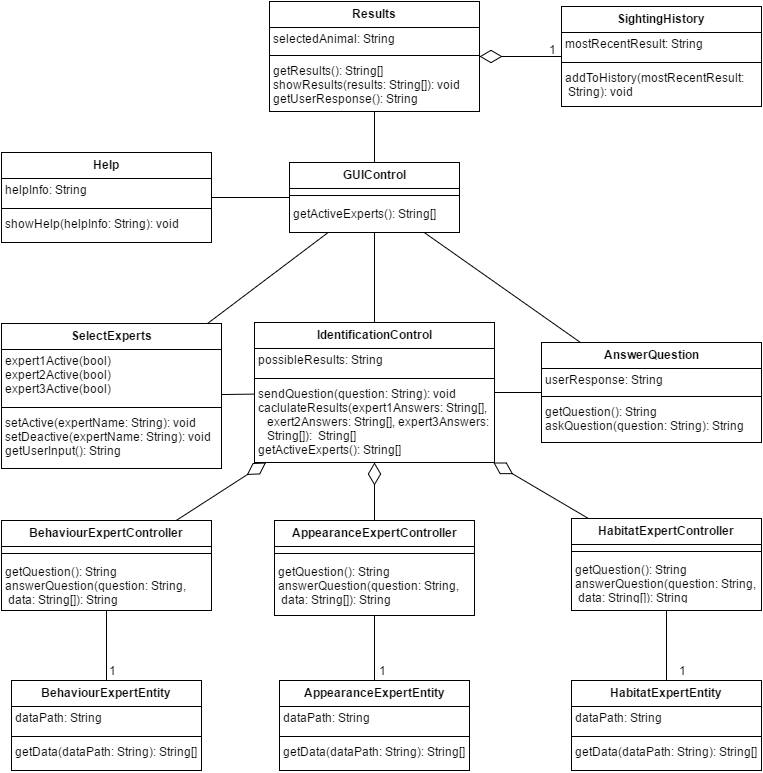
\includegraphics[width = 14cm]{DetailedClassDiagram}
	\caption{Detailed Class Diagram}
	\label{Detailed Class Diagram}
\end{figure}
% Begin Section
%This section should provide a use case diagram for your application.

% End Section


\newpage
\section*{Division of Labour}
\label{sec:division_of_labour}
\addcontentsline{toc}{section}{Division of Labour}
% Begin Section
%Include a Division of Labour sheet which indicates the contributions of each team member. This sheet must be signed by all team members.
\begin{table}[H]
	\centering
	\begin{tabular}{|p{5cm}|p{2cm}|p{3.5cm}|p{3cm}|}\hline
	    \textbf{Revisions Made} & \textbf{Date} & \textbf{Reason for Revision} & \textbf{Revising Party}\\\hline
		Added title page and introduction & 2016/03/22 & Document Creation & Alexander Jackson\\\hline
		Sequence Diagrams & 2016/03/22 & Document Addition & Josh Voskamp, Harit Patel, Mohammad Naveed\\\hline
		Added state chart diagrams & 2016/03/24 & Document Addition & Lucas Bongers\\\hline
		Created Detailed Class Diagram & 2016/03/27 & Document Addition & Harit Patel, Lucas Bongers, Alexander Jackson\\\hline
		Spelling Fixes & 2016/03/27 & Corrections & Josh Voskamp\\\hline
	\end{tabular}
\end{table}
\vspace{3cm}
\section*{Signatures}
\vspace{1cm}
\noindent Alexander Jackson \\\hrule
\vspace{1cm}
\noindent Harit Patel \\\hrule
\vspace{1cm}
\noindent Josh Voskamp \\\hrule
\vspace{1cm}
\noindent Lucas Bongers \\\hrule
\vspace{1cm}
\noindent Mohammad Naveed \\\hrule
% \section*{IMPORTANT NOTES}
% \begin{itemize}
% %	\item You do \underline{NOT} need to provide a text explanation of each diagram; the diagram should speak for itself
% 	\item Please document any non-standard notations that you may have used
% 	\begin{itemize}
% 		\item \emph{Rule of Thumb}: if you feel there is any doubt surrounding the meaning of your notations, document them
% 	\end{itemize}
% 	\item Some diagrams may be difficult to fit into one page
% 	\begin{itemize}
% 		\item It is OK if the text is small but please ensure that it is readable when printed
% 		\item If you need to break a diagram onto multiple pages, please adopt a system of doing so and thoroughly explain how it can be reconnected from one page to the next; if you are unsure about this, please ask about it
% 	\end{itemize}
% 	\item Please submit the latest version of Deliverable 1 and Deliverable 2 with Deliverable 3
% 	\begin{itemize}
% 		\item It does not have to be a freshly printed version; the latest marked version is OK
% 	\end{itemize}
% 	\item If you do \underline{NOT} have a Division of Labour sheet, your deliverable will \underline{NOT} be marked
% \end{itemize}
%

\end{document}
%------------------------------------------------------------------------------
